\documentclass[12pt, a4paper]{article}
\usepackage[normalem]{ulem}
\usepackage{xcolor}
\usepackage{amssymb}
\usepackage{graphicx}
\graphicspath{ {./images/} }\usepackage{hyperref}
\hypersetup{
    colorlinks=true,
    linkcolor=blue,
    filecolor=blue,
    urlcolor=blue,
    pdftitle={PrettyPrint Export},
    pdfpagemode=FullScreen,
    }
\urlstyle{same}
\makeatletter
\def\maxwidth#1{\ifdim\Gin@nat@width>#1 #1\else\Gin@nat@width\fi}
\makeatother

\begin{document}
\section{\texttt{PrettyPrint} in programming}
\textbf{In} \textit{programming}, \underline{PrettyPrint} \sout{refers} \texttt{to} \underline{\textbf{\textit{the}}} process of formatting or displaying the source code in an organized \& easily readable form.
 

\begin{figure}[h]
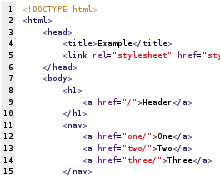
\includegraphics[width=\maxwidth{\linewidth}]{220px-HTML_source_code_example.png}
\centering
\caption{This is the Wikipedia picture for PrettyPrint as an external URL}
\end{figure}
The primary objective of PrettyPrint is to improve the code's readability by adding spacing, indentations, and line breaks while ignoring the code's semantic meaning.

\begin{itemize}
\item[ ] This is a double-nested block.

\begin{enumerate}
\item This is a first item
\begin{enumerate}
\item this a first nested item
\end{enumerate}
\item This is a second item, not worth 1\$.
\end{enumerate}
\begin{itemize}
\item[•] This is a bullet.
\end{itemize}
\begin{enumerate}
\item This is a newly numbered item.
\item[ ] This is a nested block.

\end{enumerate}
\end{itemize}
\subsection{\textcolor{red}{\underline{Code}}\underline{ Editors}}
\begin{figure}[h]
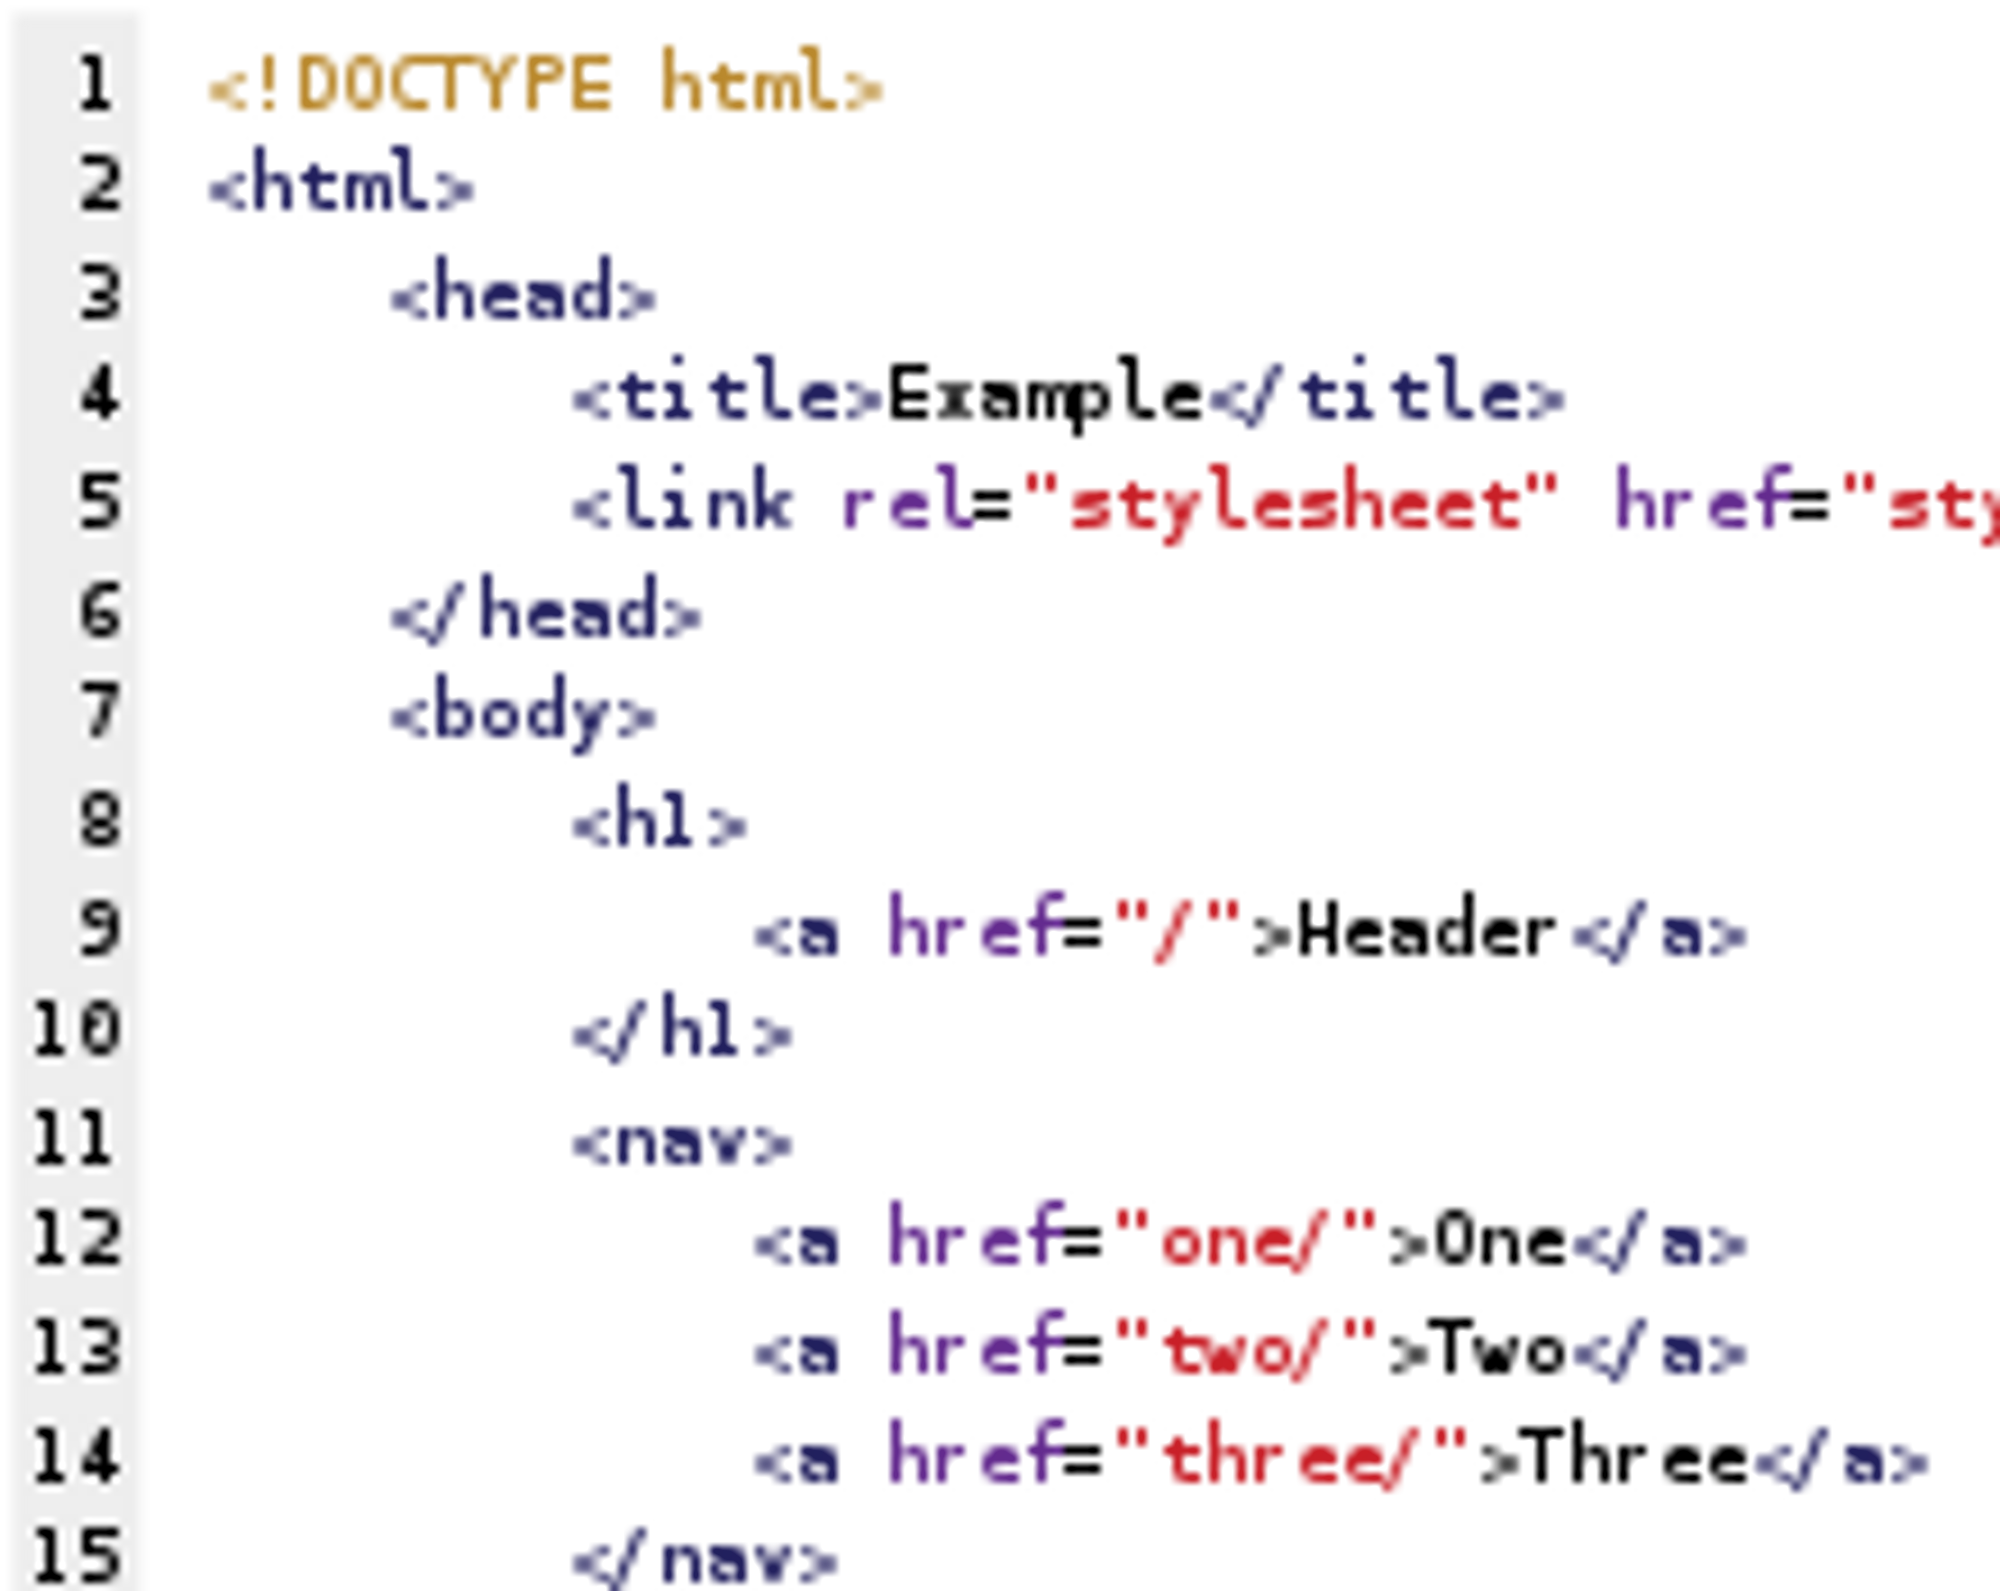
\includegraphics[width=\maxwidth{\linewidth}]{PrettyPrint.png}
\centering
\caption{This is the same picture as an uploaded file}
\end{figure}
\begin{itemize}
\item[•] PrettyPrint is an essential feature in modern code editors and integrated development environments (IDEs).
 It helps developers to analyze and debug the code quickly and efficiently.
 The formatted code is more understandable to humans, which makes it easier to spot any syntax errors, redundancies, or other issues that might arise in the code.
\begin{itemize}
\item[◦] \colorbox{pink}{In addition to improving code readability, PrettyPrint also plays a crucial role in code maintenance.
 It helps developers track the changes made to the code and compare different versions of the same code.}
\begin{itemize}
\item[$\blacksquare$] This is a sub-sub bullet.
\begin{itemize}
\item[•] This is a sub-sub-sub bullet
\end{itemize}
\end{itemize}
\end{itemize}
\item[•] Various programming languages come with their own PrettyPrint tools or libraries that enable developers to format their code automatically.
 For example, \href{http://python.org/}{Python} has a built-in \texttt{pprint} module that formats data structures in a more readable form.
 Similarly, JavaScript has a \texttt{prettier} library that formats the JavaScript code automatically.
\end{itemize}
\subsubsection{Summary}
\textcolor{red}{Overall}, \colorbox{green}{PrettyPrint} is a crucial feature in modern programming, helping developers maintain and analyze their code effectively.

\end{document}